%%%%%%%%%%%%%%%%%%%%%%%%%%%%%%%%%%%%%%%%%%%%%%%%%%%%%%%%%%%%%%%%%%%%%
%                                                                   %
%	CHAPTER ONE, CHOICES AND SPH                                    %
%                                                                   %
%%%%%%%%%%%%%%%%%%%%%%%%%%%%%%%%%%%%%%%%%%%%%%%%%%%%%%%%%%%%%%%%%%%%%
\chapter{General problem}

\section{Introduction}
In this section we give details on our choices for the generic application confronted to both computation and communication walls on irregular context. 
This problem, Smoothed Particle Hydrodynamics, is described on the physics aspect and the difficulties involved in the resolution on supercomputers.  

\section{Combining irregular behaviors}


\section{Smoothed Particle Hydrodynamics}

\subsection{General description}
Smoothed Particle Hydrodynamics (SPH) is an explicit numerical mesh-free Lagrangian method used to solve hydrodynamical partial differential equations (PDEs) by discretized it into a set of fluid elements called particles. 
This computational method was invented for the purpose of astrophysics simulations by Monaghan, Gingold and Lucy in 1977 \cite{lucy1977numerical,gingold1977smoothed}. 
This first SPH work conserved mass and they later proposed a method which also conserves linear and angular moment \cite{gingold1982kernel}. 
The method was extended for general fluid simulation and many more fields from ballistics to oceanography. 
The development of new reliable, parallel and distributed tools for this method is a challenge for future HPC architectures with the upcoming Exascale systems.

\begin{figure}
\centering
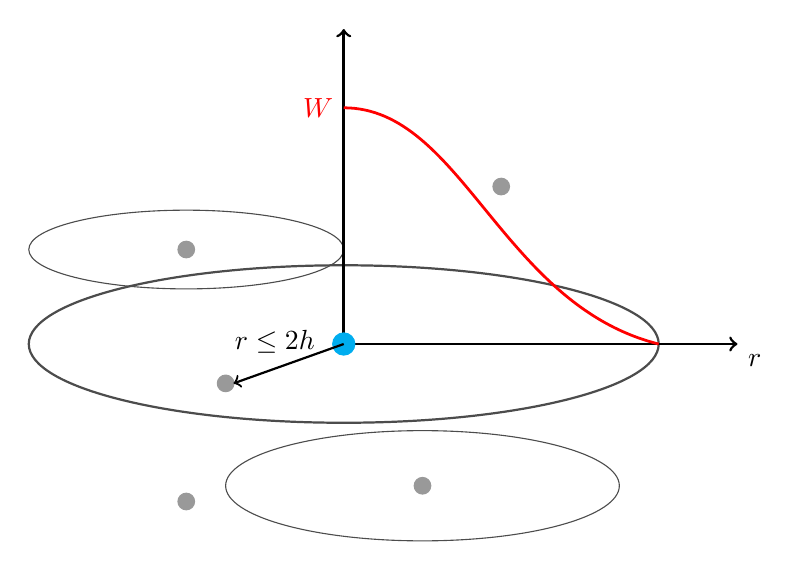
\begin{tikzpicture}
	
	% Others and their ellipse
	\draw [fill,black!40] (.5,1.5) circle (.3em);
	\draw [fill,black!40] (0,0) circle (.3em);
	\draw [fill,black!40] (0,3.2) circle (.3em);
	\draw[black!70] (0,3.2) ellipse (2 and .5);
	\draw [fill,black!40] (3,.2) circle (.3em);
	\draw[black!70] (3,.2) ellipse (2.5 and .7);
	\draw [fill,black!40] (4,4) circle (.3em);
	% Ellipses 
	\draw[line width=.8pt,black!70] (2,2) ellipse (4 and 1);
	% Axes
	\draw[->,line width=1pt] (2,2) -- (7,2) node[anchor=north west] {$r$};
	\draw[->,line width=1pt] (2,2) -- (2,6);
	% bezier for kernel 
	\draw[red,line width=1pt]  (6,2) .. controls (4,2.5) and (3.5,5) .. (2,5) node[red,anchor=east] {$W$};
	% main particle, at the end to cover
	\draw [fill,cyan] (2,2) circle (.4em);
	% Arrows 
	\draw[->,line width=.8pt] (2,2) -- (.6,1.5) node[midway, above,xshift=-.5em] {$r\leq2h$};
	
	

\end{tikzpicture}
%\includegraphics[scale=.4]{\locpath/figures/flecsph/sph.pdf}
\caption{SPH kernel $W$ and smoothing length $h$ representation}
\label{fig:sph_base}
\end{figure}

The method, as illustrated in Fig.~\ref{fig:sph_base}, computes the evolution of physical quantities for every particle regarding its neighbors in the radius of its smoothing length $h$. 
The particles in this radius are then valued according to their distance using a smoothing function $W$, also called a kernel. 
The fundamental SPH formulation for any physical quantity $A$ is then to compute with all the neighbors of $b$ of a particle by:
\begin{equation}
A(\vec{r}) \simeq \sum_b \frac{m_b}{\rho_b} A(\vec{r}_b) W ( |\vec{r}-\vec{r}_b|,h)
\end{equation}

On a physics aspect, this method has several advantages:
It can handle deformations, low densities, vacuum, and makes particle tracking easier. 
It also conserves mass, linear and angular momenta, and energy by its construction that implies independence of the numerical resolution. 
Another strong benefit of using SPH is its exact advection of fluid properties. 
Furthermore, the particle structure of SPH easily combines with tree methods for solving Newtonian gravity through N-body simulations.
As a mesh-free method, it avoids the need of grid to calculate the spatial derivatives. 

However, there are cons to consider using SPH: 
It is restricted to low-order rate of convergence on certain PDE formulations; 
It requires careful setup of initial distribution of particles; 
Further, it can be struggle to resolve turbulence-dominated flows and special care must be taken when handling high gradients such as shocks and surface structure of neutron stars.
Many works are leading to handle more cases and to push the limitations of this method \cite{dai2017dual,lind2016incompressible,ren2016dual}.

In this work, we are solving Lagrangian conservation equations (Euler equations) for mass, energy and momentum of an ideal fluid ~\cite{Landau1959}  such that:
\begin{equation}
\frac{d \rho}{d t} = - \rho \nabla \cdot \vec{v}, \quad
\frac{d u}{d t} = \left( \frac{P}{\rho^2} \right) \frac{d \rho}{d t}, \quad
\frac{d \vec{v}}{d t} = - \frac{\nabla P}{\rho}
\end{equation}
with $\rho$ the density, $P$ the pressure, $u$ the internal energy and $v$ the velocity, where $d/dt = \partial_t + \vec{v} \cdot \nabla$ which is convective derivative.

By using the volume element $V_b = m_b / \rho_b$, we can formulate the Newtonian SPH scheme~\cite{rosswog2009} such that
\begin{equation}
\label{eq:rho}
\rho_a = \sum_b m_b W_{ab} (h_a)
\end{equation}
\begin{equation}
\frac{d u_a}{dt} = \frac{P_a}{\rho_a^2} \sum_b m_b \vec{v}_{ab} \cdot \nabla_a W_{ab} 
\end{equation}
\begin{equation}
\frac{d \vec{v}_a}{d t} = - \sum_b m_b \left(\frac{P_a}{\rho_a^2} + \frac{P_b}{\rho_b^2} \right) \nabla_a W_{ab}
\end{equation}
where $W_{ab} = W(| \vec{r}_a - \vec{r}_b |,h)$ is the smoothing kernel. 
The equations we would like to solve allow for emergence of discontinuities from smooth initial data. 
At discontinuities, the entropy increases in shocks. That dissipation occurs inside the shock-front. 
The SPH formulation here is inviscid so we need to handle this dissipation near shocks. 
There are a number of way to handle this problem, but the most widespread approach is to add artificial viscosity (or artificial dissipation) terms in SPH formulation such that:
\begin{equation}
\left(\frac{d u_a}{dt} \right)_{art} = \frac{1}{2} \sum_b m_b \Pi_{ab} \vec{v}_{ab} \cdot \nabla_a W_{ab}
\end{equation}
\begin{equation}
\left(\frac{d\vec{v}_a}{dt} \right)_{art} = - \sum_b m_b \Pi_{ab}\nabla_a W_{ab}
\end{equation}
In general, we can express the equations for internal energy and acceleration with artificial viscosity
\begin{equation}
\label{eq:intern}
\frac{d u_a}{dt} = \sum_b m_b \left(\frac{P_a}{\rho_a^2} + \frac{\Pi_{ab}}{2} \right) \vec{v}_{ab} \cdot \nabla_a W_{ab}
\end{equation}
\begin{equation}
\label{eq:velo}
\frac{d \vec{v}_a}{d t} = - \sum_b m_b \left(\frac{P_a}{\rho_a^2} + \frac{P_b}{\rho_b^2} + \Pi_{ab} \right) \nabla_a W_{ab}
\end{equation}
$\Pi_{ab}$ is the artificial viscosity tensor. 
As long as $\Pi_{ab}$ is symmetric, the conservation of energy, linear and angular momentum is assured by the form of the equation and antisymmetry of the gradient of kernel with respect to the exchange of indices $a$ and $b$. $\Pi_{ab}$ may define different way but here we use~\cite{Monaghan1983} such as: 
\begin{equation}
\Pi_{ab} = \begin{cases}
\frac{- \alpha \bar{c}_{ab} \mu_{ab} + \beta \mu_{ab}^2}{\bar{\rho}_{ab}} & \text{for $\vec{r}_{ab} \cdot \vec{v}_{ab} < 0$} \\
0 & \text{otherwise}
\end{cases}
\end{equation}
\begin{equation}
\mu_{ab} = \frac{\bar{h}_{ab} \vec{r}_{ab} \cdot \vec{v}_{ab}}{r^2_{ab} + \epsilon \bar{h}_{ab}^2}
\end{equation}

Using the usual form $c_s$ as $c_s = \sqrt{\frac{\partial p}{\partial \rho}}$.
The values of $\epsilon$, $\alpha$, and $\beta$ have to be set regarding the problem targeted. 
Here, we use $\epsilon = 0.01h^2$, $\alpha = 1.0$, and $\beta = 2.0$. 

There are many possibilities for the smoothing function, called the kernel. 
As an example the Monaghan's cubic spline kernel is given by:
\begin{equation}
W(\vec{r},h) = \frac{\sigma}{h^D} \begin{cases}
1-\frac{3}{2} q^2 + \frac{3}{4} & \text{if} \indent 0 \leq q \leq 1 \\
\frac{1}{4} (1-q)^3  & \text{if} \indent 1 \leq q \leq 2 \\
0 & \text{otherwise}
\end{cases}
\end{equation}
where $q = r/h$, $r$ the distance between the two particles, $D$ is the number of dimensions and $\sigma$ is a normalization constant with the values:
\begin{equation}
\sigma =  \begin{cases}
\frac{2}{3} & \text{for 1D}  \\
\frac{10}{7 \pi} & \text{for 2D} \\
\frac{1}{\pi} & \text{for 3D}
\end{cases}
\end{equation}

To sum up, the SPH resolution scheme and its routines are presented on algorithm \ref{alg:sph}.
The Equation of State (EOS) and the integration are problem dependent and will be define for each test case in section \ref{sec:applications}. 

\begin{algorithm}
\caption{SPH loop algorithm}\label{alg:sph}
\begin{algorithmic}[1]
\While{not last step}
\State Compute density for each particle (\ref{eq:rho})
\State Compute pressure using EOS 
\State Compute acceleration from pressure forces (\ref{eq:velo})
\State Compute change of internal energy for acceleration (\ref{eq:intern})
\State Advance particles after integration
\EndWhile
\end{algorithmic}
\end{algorithm}

The main downside for the implementation of this method is the requirement for local computation on every particle. 
The particles have to be grouped locally to perform the computation of (\ref{eq:rho}), (\ref{eq:intern}) and (\ref{eq:velo}).
A communication step is needed before and after (\ref{eq:rho}) to get the local physical data to be able to compute (\ref{eq:intern}) and (\ref{eq:velo}).
The tree data structure allows us to perform $O(Nlog(N))$ neighbor search but also add a domain decomposition and distribution layer.

As the SPH method is used in a large panel of fields from astrophysics to fluid mechanic, there are numerous related works. 
We can cite a code developed in the LANL, 2HOT \cite{warren20132hot} that introduced the Hashed Oct Tree structure used in our implementation. 
There is also GADGET-2 \cite{springel2005cosmological}, GIZMO \cite{hopkins2014gizmo} and the most recent publication is GASOLINE \cite{wadsley2017gasoline2} based on PKDGRAV, a specific tree+gravity implementation. 
Several implementations already implement GPU code and tree construction and traversal, one can cite GOTHIC \cite{miki2017gothic}, presenting gravitational tree code accelerated using the latest Fermi, Kepler and Maxwell architectures. But a lot of GPU accelerated work still focused on fluid problems and not on astrophysical problems  \cite{harada2007smoothed,crespo2011gpus}.
We also note that these implementations focus on SPH problems and does not provide a general purpose and multi-physics framework like we intent to provide through FleCSPH and FleCSI. 

\subsection{Gravitation}
For classical problems like fluid flow the gravitation can directly be applied on the particles with the force:
\begin{equation}
	\vec{a_g} = m\vec{g}
\end{equation}

In order to consider astrophysics problems we need to introduice self-gravitation. 
Each particle imply an action on the others base on its distance and mass. 
The equation of gravitation for a particle $i$ with $j$ other particles is: 
\begin{equation}
	\vec{f_a}_i = \sum_j -G \frac{m_i m_j}{|\vec{r_i}-\vec{r_j}|^3} \vec{r_{ij}}
	\label{eq:gravitation}
\end{equation}

This computation involve an $O(N^2)$ complexity and thus is not applicable directly. 
We applied the method called Fast Multipole Method, FMM and discussed in \cite{beatson1997short}.
In this method we compute the gravitation up a approximations. 
The user can refine those approximation changing parameters. 

This method is based on Taylor series.
The gravitation function of equation~\ref{eq:gravitation} can be approximate on a particle at position $\vec{r}$ by the gravitation computed at the centroid at position $\vec{r_c}$: 
\begin{equation}
 \vec{f}(\vec{r}) = \vec{f}(\vec{r_c}) + ||\frac{\partial\vec{f}}{\partial\vec{r}}||\cdot (\vec{r} - \vec{r_c}) + \frac{1}{2} (\vec{r}-\vec{r_c})^\intercal \cdot   ||\frac{\partial\vec{f}}{\partial\vec{r} \partial\vec{r}}|| \cdot (\vec{r} - \vec{r_c})
 \end{equation}

 From equation~\ref{eq:gravitation} we compute the term $||\frac{\partial\vec{f}}{\partial\vec{r}}||$:s
 \begin{equation}
\frac{\partial\vec{f}}{\partial\vec{r}} =
- \sum_p \frac{m_p}{|\vec{r_c}-\vec{r_p}|^3}
\begin{bmatrix}
1 - \frac{3(x_c-x_p)(x_c-x_p)}{|\overline{r_c}-\overline{r_p}|^2} & -\frac{3(y_c-y_p)(x_c-x_p)}{|\overline{r_c}-\overline{r_p}|^2}  & -\frac{3(z_c-z_p)(x_c-x_p)}{|\vec{r_c}-\vec{r_p}|^2}  \\
-\frac{3(x_c-x_p)(y_c-y_p)}{|\vec{r_c}-\vec{r_p}|^2}  & 1 - \frac{3(y_c-y_p)(y_c-y_p)}{|\vec{r_c}-\vec{r_p}|^2} &  -\frac{3(z_c-z_p)(y_c-y_p)}{|\vec{r_c}-\vec{r_p}|^2}\\
- \frac{3(x_c-x_p)(z_c-z_p)}{|\vec{r_c}-\vec{r_p}|^2}   &  -\frac{3(y_c-y_p)(z_c-z_p)}{|\vec{r_c}-\vec{r_p}|^2} &  1- \frac{3(z_c-z_p)(z_c-z_p)}{|\vec{r_c}-\vec{r_p}|^2} \\
\end{bmatrix}
 \end{equation}

And we propose a compact version of the matrix with: 
 
\begin{equation}
 ||\frac{\partial f^a}{\partial r^b}|| = -\sum_c \frac{m_c}{|\vec{r}-\vec{r_c}|^3} \Big[ \delta_{ab} - \frac{3.(r^a-r_c^a)(r^b-r_c^b)}{|\vec{r}-\vec{r_c}|^2} \Big] 
\end{equation}

With $\delta_{ij}$ the kronecker delta:
\begin{equation}
\delta_{ij} = 
\begin{cases}
    1, & \text{if $i = j$}.\\
    0, & \text{if $i\neq j$}.
  \end{cases}
\end{equation}

We note that $a$ and $b$ variate from 0 to 2 and $r^0=x$, $r^1=y$, and $r^2=z$ as usual sense. 

For the term $||\frac{\partial\vec{f}}{\partial\vec{r} \partial\vec{r}}||$ we give the compact version by:
\begin{equation}
||\frac{\partial^2 f^a}{\partial r^b \partial r^c}|| =
- \sum_c \frac{3 m_c}{|\vec{r}-\vec{r_c}|^5} \left[\frac{5(r^a-r_c^a)(r^b-r_c^b)(r^c-r_c^c)}{|\vec{r}-\vec{r_c}|^2} - \left( \delta_{ab} (r^c-r_c^c)+\delta_{bc} (r^a-r_c^a)+\delta_{ac} (r^b-r_c^b) \right) \right] 
 \end{equation} 

 \begin{figure}
 \end{figure}

The method is summed up in figure with the different equations.
We consider Centers Of Mass, COM, to be the centroid of particles based on their position. 
In several steps the information is first transmetted to the COMs, computing their position and mass. 


\subsection{Problems} 

\subsubsection{Sod shock tube}

\subsubsection{Sedov blast wave}

\subsubsection{Fluid flow}

\subsubsection{Astrophysics: neutron stars coalescing}

\section{Conclusion}
